\documentclass[laurea,oneside,11pt]{USiena_tesiLM}
\usepackage{amsfonts}
\usepackage{amssymb}
\usepackage[italian]{babel}
\usepackage[T1]{fontenc} 
\usepackage{graphicx} % Required for the inclusion of images
\usepackage[normal]{subfigure}

\usepackage[utf8]{inputenc}
\usepackage[swapnames,signatures]{frontespizio}
%\usepackage{fancyhdr}


%
\pagestyle{headings} % oppure fancy
%\renewcommand{\headrulewidth}{0.5pt}
%\fancyhf{}
%\fancyhead[LE,RO]{\thepage}
%\fancyhead[RE,LO]{\rightmark}

%
%pagina bianca
%
\newcommand{\facciatabianca}{\newpage\shipout\null\stepcounter{page}}

%% QUESTA PARTE E' MOLTO IMPORTANTE
%%PER INSERIRE LE CORRETTE IMPOSTAZIONI PERSONALI
%%
%% Titolo ed autore
%\title{Come strutturare la tesi di laurea magistrale}
%\author{Marco Becattini\\~\\}
%\date{8 Febbraio 2016}
%\titolocorso{Computer and Automation Engineering\\curricula: Robotics and Automation}
%\degreeyear{2015/2016}
%% Relatore principale
%\chair{Prof. A. Vicino \medskip}
%%
%% Coordinatore
%\othermembers{}
%%Altri relatori
%\othermembers{Prof. A. Giannitrapani\medskip\\Prof. S. Paoletti\medskip\\}
%\numberofmembers{3}  % Numero dei relatori
%%
%
%
%\def\BibTeX{{\rm B\kern-.05em{\sc i\kern-.025em b}\kern-.08em
%    T\kern-.1667em\lower.7ex\hbox{E}\kern-.125emX}}

%%%%%%%%%%%%%%%%%%%%%%%%%%%%%%%%%%%%%%%%%%%%%%%%%%%%%%%%%%%
\begin{document}

\begin{frontespizio}
%% This file has been automatically generated by `frontespizio'.
%% Don't use it as a model for a new frontispiece, use the
%% `frontespizio' environment in you document instead.
\Universita {Siena}
\Logo [4cm]{logosm.jpg}
\Facolta {Ingegneria}
\Dipartimento {Ingegneria dell’Informazione e Scienze Matematiche}
\Corso [Laurea Magistrale]{Computer and Automation Engineering\\curricula: Robotics and Automation}
\Annoaccademico {2015-2016}
\Titoletto {Tesi di Laurea Magistrale}
\Titolo {Simulazione e ottimizzazione dei consumi di un impianto di teleriscaldamento alimentato da fonte geotermica}
\Sottotitolo {}
\Candidato {Marco Becattini}
\Relatore {Prof. A. Vicino}
\Correlatore {Prof. A. Giannitrapani}
\Correlatore {Prof. S. Paoletti}
\Margini {3cm}{2cm}{3cm}{2cm}
\end{frontespizio}

\facciatabianca


%
%\maketitle                  % pagina del titolo
%
\begin{abstract}          % Pagina del sommario
  This is a LaTeX2e style for writing thesis. It is based on the
  book LaTeX2e class. The abstract is not present on the original
  book class, it is taken from the report class.
  The bastract is single spaced.
\end{abstract}             % pagina del sommario

%%%%%%%%%%%%%%%%%%%%%%%%%%%%%%%%%%%%%%%%%%
% parte iniziale
% Nel frontespizio la numerazione
% \`{e} romana e le intestazioni sono semplici
%%%%%%%%%%%%%%%%%%%%%%%%%%%%%%%%%%%%%%%%%%%%
\frontmatter
Ringraziamenti            % ringraziamenti
\
%\input{dedica}
\tableofcontents            % indice
%\listoffigures            % indice delle figure
%\listoftables              % indice delle tabelle
%


%%%%%%%%%%%%%%%%%%%%%%
% parte principale
%%%%%%%%%%%%%%%%%%%%%%
\mainmatter

\chapter*{Introduzione}
\markboth{Introduzione}{Introduzione}
La geotermia costituisce una risposta alle esigenze di salvaguardia ambientale e di sviluppo sostenibile: è una fonte che lavora in maniera costante sfruttando il calore naturale della terra.
Il termine "geotermia" deriva dal greco e significa letteralmente calore della Terra. Per energia geotermica si intende, quindi, l'energia contenuta sotto forma di calore all'interno del nostro pianeta. Di fatto, però, è possibile utilizzare industrialmente solo il calore che si trova concentrato in alcune zone privilegiate, dove sono presenti masse magmatiche fluide o in via di raffreddamento. La risorsa geotermica disponibile a profondità accessibili è contenuta in un serbatoio naturale sotto forma di vapore o acqua a elevata temperatura, in gran parte piovana, che si riscalda circolando nelle rocce calde e permeabili. Se vi sono fratture nella crosta terrestre (faglie) o affioramenti di rocce permeabili, nel raggiungere la superficie, acqua e vapore possono dar luogo a manifestazioni naturali spettacolari come geyser, lagoni, fumarole.
La prima utilizzazione dell'energia geotermica, per la produzione di energia elettrica, avvenne il 4 luglio 1904 in Italia per merito del principe Piero Ginori Conti che sperimentò il primo generatore geotermico a Larderello in Toscana preludio delle vere e proprie centrali geotermiche. 
L'energia geotermica, inoltre, viene usata anche per la produzione di energia termica. Un sistema che sfrutta la geotermia per la produzione di calore e la sua distribuzione  ai centri abitati è il teleriscaldamento. Il teleriscaldamento è  un  servizio  di  distribuzione  urbana  del calore per  riscaldamento di ambienti e produzione di acqua calda sanitaria con produzione centralizzata. Il calore viene trasportato attraverso una rete di tubazioni interrate di acqua calda, acqua surriscaldata o vapore, detti fluidi termovettori, proveniente da una grossa centrale di produzione, alle abitazioni con successivo ritorno dei suddetti alla stessa centrale.
In particolare nel comune di Pomarance, comune italiano della provincia di Pisa storicamente importante per lo sviluppo e lo sfruttamento dell'energia geotermica nella frazione di Larderello,l'azienda Geo Energy Service s.p.a. (G.E.S. s.p.a.) nata nel luglio del 2006, si occupa della gestione delle centrali termiche e delle relative reti di teleriscaldamento. In tutto gestisce nove centrali termiche alimentate da energia geotermica e sei reti di teleriscaldamento che si estendono per $200 \ km$, per un totale di $2.400$ utenze allacciate con una volumetria di circa $800.000 \ m^3$ erogando energia per circa $45.000 \ Gcal/anno$. 
A fronte dell'aumento, negli ultimi anni, del numero di utenze allacciate alla rete di distribuzione del calore, si è notato come i costi di gestione degli impianti sia cresciuto notevolmente a causa di inefficienze dovute alla mancanza di elementi di controllo e corrette regolazioni per l'ottimizzazione dell'intero sistema.
Lo scopo del seguente elaborato è stato quello di cercare delle soluzioni per massimizzare l'efficienza energetica e diminuire i costi di gestione di un impianto di teleriscaldamento da fonte geotermica. In un impianto di teleriscaldamento alimentato da fonte di calore geotermica gli unici consumi di energia non rinnovabile  derivano dalla energia elettrica consumata  per il pompaggio delle acque di circolazione. 
Le stazioni di pompaggio lavorano a regime variabile e per una ottimizzazione del sistema, bisogna far si che le pompe lavorino sempre in condizioni di buon rendimento e con il minimo dei consumi , questo vuol dire far circolare la minima quantità possibile di acqua e far si che le temperature di ritorno siano le più basse possibili. Se nella rete di distribuzione non vi sono regolazioni presso le utenze, come l'assenza di centraline d'utenza, tutta la portata circola nei primi scambiatori e per alimentare gli ultimi si deve pompare un maggior quantitativo di acqua, inoltre, le temperature di ritorno delle prime utenze saranno più alte. Le centraline di utenza ben realizzate risultano essere un elemento fondamentale per la regolazione e l'ottimizzazione di un impianto di teleriscaldamento in quanto possono  limitare la portata dell'utenza allo stretto indispensabile e limitare al massimo la temperatura di ritorno alla centrale di scambio. Più le temperature di ritorno sono basse più energia si riesce a trasferire a pari portata . Le centraline di utenza sono inoltre il luogo dove si possono rilevare molte informazioni utili per l'ottimizzazione del circuito ad esempio le condizioni di arrivo dei fluidi nei punti estremi del circuito non facilmente prevedibili istante per istante in quanto dipendono dalle richieste del momento di tutte le utenze precedenti .
Dalle centraline si possono fare anche analisi di predittiva sullo stato di funzionamento degli scambiatori con segnalazione di anomalie che portano ad interventi programmati invece che in accidentale .
Le centraline di utenza "intelligenti " possono inoltre aiutare i proprietari degli immobili a fare efficienza ed a evitare picchi di consumo sul circuito .
Tutte le soluzioni studiate, sono state simulate in ambiente \textsc{Matlab} e confrontate con dati reali misurati sul campo.

\textit{Scrivere breve riassunto su ogni capitolo}

\chapter{Geotermia e Teleriscaldamento}

\chapter{Tecnologie degli impianti di teleriscaldamento}
%\label{Capitolo3}
Un impianto di teleriscaldamento è un  sistema di riscaldamento a distanza di un quartiere o di una città 
che utilizza il calore prodotto da una centrale termica, da un impianto di cogenerazione 
o da una sorgente geotermica distribuendolo agli edifici tramite una rete di tubazioni in cui fluisce l'acqua calda che verrà utilizzata per la produzione di acqua igienico sanitaria e il riscaldamento di edifici residenziali e commerciali.  \\
Le componenti principali di un sistema di teleriscaldamento sono come riportato in figura \ref{fig:schema1}: una centrale termica, dove viene prodotto il calore, una rete di distribuzione, costituita da tubazioni 
coibentate interrate, e un insieme di sotto-centrali. Queste ultime, situate nei singoli 
edifici da servire, sono costituite da scambiatori di calore, che permettono di realizzare 
lo scambio termico tra il fluido termovettore  della rete primaria del teleriscaldamento con l'acqua del circuito delle utenze, senza che vi sia così miscelazione tra i due fluidi semplificando quindi di molto la progettazione dell'intera rete. Lo scambiatore infatti andrà semplicemente a sostituire la  caldaia convenzionale mantenendo invariato l'impianto già esistente dell'utenza.

\begin{figure}[h]
\begin{center}
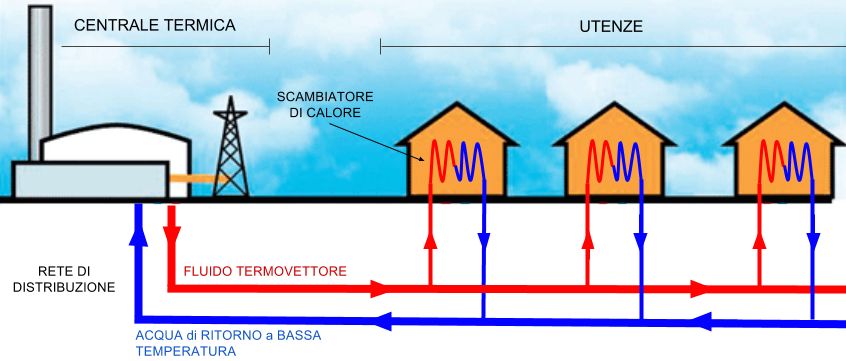
\includegraphics[width=1.0\textwidth]{figure/schema_impianto1}
\caption{Schema di un impianto di teleriscaldamento composto da: centrale di scambio, rete di distribuzione e sotto-centrali di scambio (scambiatori)}
\label{fig:schema1}
\end{center}
\end{figure}

La centrale termica riscalda l'acqua che viene distribuita ai diversi edifici attraverso la rete di distribuzione con l'ausilio di pompe. Giunta allo scambiatore, l'acqua della rete trasferisce all'acqua dell'impianto di distribuzione interno dell' edificio, il calore necessario per riscaldare gli ambienti e per la produzione di acqua calda sanitaria. L'acqua, ormai raffreddata, ritorna in centrale per essere nuovamente riscaldata. 
%Il teleriscaldamento riesce ad essere economicamente conveniente a patto che si riesca a trovare un bacino di utenze concentrate in un'area relativamente ridotta. La traduzione inglese di teleriscaldamento "district heating" che letteralmente tradotta vuol dire "riscaldamento distrettuale", rende l'idea della concentrazione che l'utenza 
%dovrebbe avere per far sì che questo metodo sia economicamente vantaggioso. \\
In seguito si analizzerà più approfonditamente ogni elemento dell'impianto.

\section{Centrale termica e di scambio}
Le centrali termiche, analizzate nell'elaborato, sfruttano il vapore geotermico non idoneo alla generazione di energia elettrica. Le centrali di scambio si occupano dello scambio di calore tra due diversi circuiti. La centrale termica può essere interpretata come una centrale di scambio in quanto non fa altro che estrarre dal vapore l'energia termica necessaria per l'intero impianto di teleriscaldamento. Il vapore, dunque, arriva in centrale a circa $240 ^{\circ}C$ e cede la sua energia termica attraverso gruppi di scambio termico costituito da uno scambiatore vapore-acqua surriscaldata a circa $120 ^{\circ}C$ e da un desurriscaldatore di condensa acqua acqua. La portata del vapore è controllata attraverso  valvole a due vie di tipo NC, in funzione della temperatura  di uscita dell'acqua surriscaldata nel circuito primario. La condensa viene raccolta in un serbatoio atmosferico e reiniettata nel punto di raccolta gestito da ENEL con pompe centrifughe multistadio, in modo da mantenere e rinnovare la risorsa geotermica. L'acqua surriscaldata viene inviata attraverso una linea feeder ad una seconda centrale di scambio, posta nei pressi del centro abitativo, dove cede la sua energia termica attraverso gruppi di scambio termico costituiti da uno scambiatore acqua surriscaldata - acqua calda. La portata di acqua surriscaldata è controllata attraverso valvole a due vie di tipo NC, in funzione della temperatura in uscita dell'acqua calda che varia tra gli $80-90 ^{\circ}C$ nel circuito secondario. Questo ulteriore scambio permette di separare la linea dell'acqua surriscaldata  dai circuiti urbani, che sono più estesi, riducendo così la potenza dell'impianto di pompaggio, le perdite di calore e il costo della rete. Inoltre, l'utilizzo di acqua calda anziché surriscaldata nei centri urbani, aumenta il livello di sicurezza e riduce gli interventi di manutenzione dovuti alla maggiore complessità degli impianti di utenza ad acqua surriscaldata. La circolazione sia nel circuito primario che secondario sono garantite da elettropompe centrifughe ubicate nella stessa centrale di scambio [figura \ref{fig:schema2}].
Nel caso in cui la centrale termica si trovi nei pressi delle utenze sarà possibile omettere la seconda centrale di scambio ed effettuare direttamente uno scambio di calore da vapore ad acqua calda [figura \ref{fig:schema3}].
%\begin{figure}[h]
%\begin{center}
%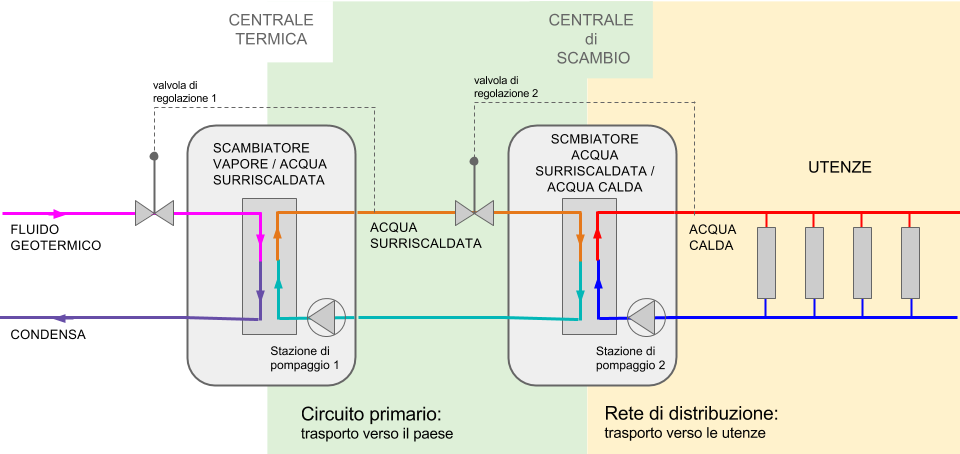
\includegraphics[width=1.0\textwidth]{figure/schema_impianto2}
%\caption{Schema impianto di teleriscaldamento con due stazioni di scambio}
%\label{fig:schema2}
%\end{center}
%\end{figure}

%\begin{figure}[h]
%\begin{center}
%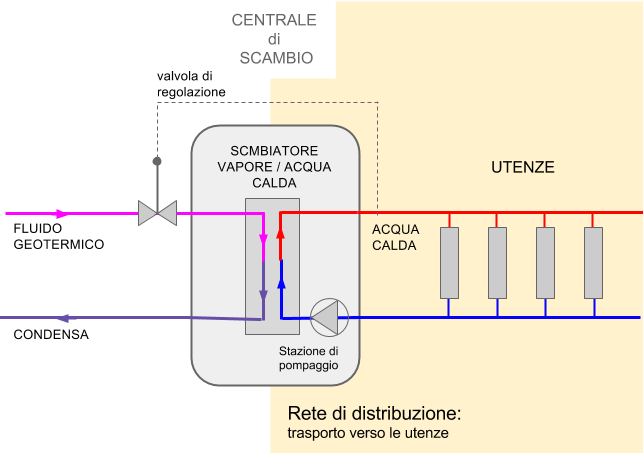
\includegraphics[width=1.0\textwidth]{figure/schema_impianto3}
%\caption{Schema impianto di teleriscaldamento con singola stazione di scambio}
%\label{fig:schema3}
%\end{center}
%\end{figure}

 \begin{figure}[h]
 \centering
 \subfigure[Schema di un impianto di teleriscaldamento con due centrali di scambio. Questa configurazione è utilizzata quando la centrale termica è distante dal centro abitativo.\label{fig:schema2}]
   {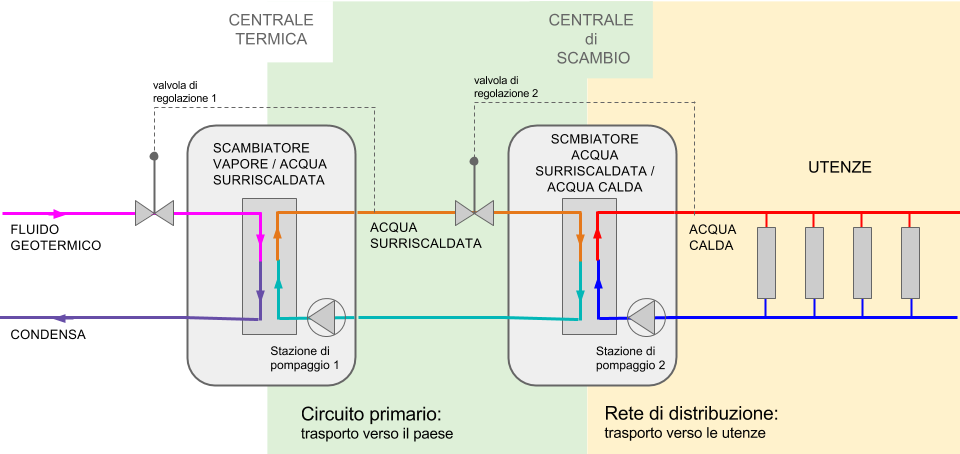
\includegraphics[width=12.5cm]{figure/schema_impianto2}}
 \hspace{5mm}
 \subfigure[Schema di un impianto di teleriscaldamento con singola centrale di scambio.\label{fig:schema3}]
   {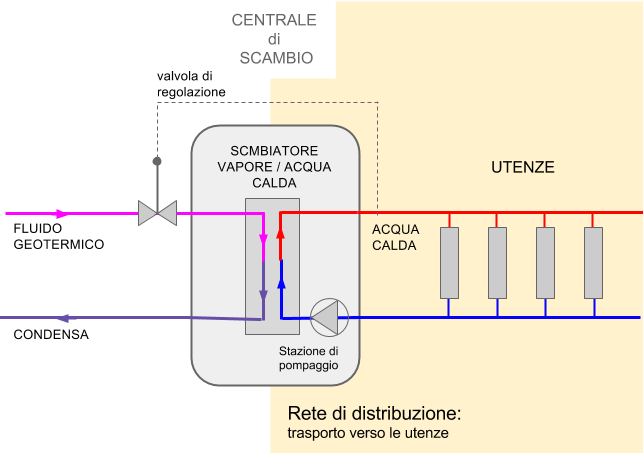
\includegraphics[width=8.5cm]{figure/schema_impianto3}}
 \caption{Possibili configurazioni di un impianto di teleriscaldamento alimentato da fonte geotermica}
 \end{figure}


\section{Stazioni di Pompaggio}
Le stazioni di pompaggio lavorano a regime variabile e sono gli elementi responsabili dei consumi di un impianto di teleriscaldamento. Risulta dunque fondamentale avere una regolazione per evitare lo spreco di energia di pompaggio. 
Nel caso vi siano due stazioni di pompaggio, e quindi due centrali di scambio, possiamo regolare  sia le pompe che alimentano il circuito primario che quelle della rete di distribuzione. Le pompe che alimentano il circuito primario sono regolate in base al grado di laminazione della valvola nella seconda centrale di scambio, la quale garantisce che la temperatura dell'acqua in mandata nella rete di distribuzione rimanga costante al valore desiderato.  Più che la valvola risulta laminata più che aumenta la resistenza idraulica sul circuito primario, portando, di conseguenza, ad una riduzione della portata e ad un aumento della prevalenza nel circuito. La regolazione delle pompe che alimentano la rete di distribuzione dipendono dalle diverse esigenze di utilizzo idrico durante l'arco della giornata. 
In impianti dove è presente una sola centrale di scambio l'unica taratura verrà effettuata sulla velocità delle pompe che inviano acqua nella rete di distribuzione affinché tutte le utenze possano usufruire della portata necessaria per soddisfare il proprio fabbisogno termico.
Dal momento che gli elementi che dovrebbero fornire informazioni sulla regolazione della velocità delle pompe si  trovano in luoghi diversi e distanti rispetto al posizionamento delle stazioni di pompaggio, sono adottati i seguenti metodi di regolazione della potenza delle pompe:
\begin{enumerate}
\item Regolazione a pressione costante
\item Regolazione a differenza di temperatura costante
\end{enumerate}

\subsection{Regolazione a pressione costante}
Nel seguente tipo di regolazione viene misurata la pressione in mandata del circuito primario e la pressione sul ritorno dello stesso circuito.  Laminando la valvola di regolazione otteniamo una dispersione di energia sulla valvola stessa tanto più grande tanto è maggiore il suo livello di chiusura. La laminazione comporta un aumento della resistenza idraulica e lo spostamento del punto di funzionamento della pompa. Il fenomeno è descritto in figura \ref{fig:dP}.

Con i sistemi di regolazione  a pressione costante la pompa in servizio viene pilotata a velocità variabile mediante un convertitore di frequenza (Inverter). La velocità di rotazione dell'elettropompa viene adeguata istantaneamente in base alla pressione differenziale di erogazione impostata. Il punto di funzionamento perciò si posizionerà sulla retta orizzontale che definisce la variazione di prevalenza $\Delta H$ di set-point, rendendo necessario far lavorare la pompa a giri ridotti riducendo i consumi.

$P_1$, il punto di funzionamento con valvola tutta aperta con portata $G_1$ e prevalenza $H_1$. Chiudendo la regolazione la resistenza idraulica aumenta facendo alzare più velocemente la curva caratteristica dell'impianto primario spostando il punto di funzionamento in $P_2$ con portata  $G_2$ e prevalenza $H_2$. 


\subsection{Regolazione a differenza di temperatura costante}

\section{Rete di distribuzione}
La rete di distribuzione è la linea che trasporta acqua calda alle utenze verso le sotto-centrali di scambio. La rete è composta da tubazioni interrate che  devono  essere adeguatamente isolate  in  modo  da  evitare  che  la temperatura  del fluido termovettore si abbassi troppo lungo il tragitto. 
Il  lemma  inglese  stesso,  district  heating,  indica  l'importanza  che  ha  il  fattore  di localizzazione  di un sistema  di  teleriscaldamento, infatti,  l'area  teleriscaldabile  deve  essere  preferibilmente  un distretto  urbano,  cioè  un'area  ad  alta  densità  abitativa,  dove  le  costruzioni  sono abbastanza concentrate.
Aree  con  edifici  troppo  isolati  tra  loro  non  sono  infatti  convenienti  da  teleriscaldare, poiché
la rete di tubazioni si estenderebbe troppo e aumenterebbero le dispersioni di calore.
I terminali della rete di distribuzione sono le sotto-centrali di scambio (scambiatori). Da un punto di vista idraulico gli scambiatori di utenza vengono visti come una resistenza variabile che definiscono la caratteristica dell'impianto. 
Se nella rete di distribuzione non vi sono regolazioni sulla portata in ingresso alla sotto-centrale di scambio delle utenze, tutta la portata circolerà nei primi scambiatori e per alimentare gli ultimi si dovrà pompare un maggior quantitativo di acqua. Inoltre, avendo le prime utenze un surplus in portata, il calore disponibile sarà di gran lunga superiore a quello necessario perciò si scambierà solo una piccola parte di energia con la conseguenza che le temperature di ritorno saranno più alte.
L'introduzione di centraline di utenza, ovvero di elementi che regolano la portata in ingresso allo scambiatore in base calore necessario all'utenza, risultano fondamentali per l'ottimizzazione di un impianto.  Centraline d'utenza ben configurate dovrebbero assicurare:
\begin{itemize}
\item limite sulla portata allo stretto indispensabile
\item riduzione delle temperature di ritorno dello scambiatore
\item aiutare l'utilizzatore a fare efficienza ovvero ridurre i consumi
\end{itemize} 
Questi elementi di regolazione sono inoltre un luogo dove si possono rilevare molte informazioni utili per l'ottimizzazione del circuito ad esempio le condizioni di arrivo dei fluidi nei punti estremi della rete non facilmente prevedibili istante per istante in quanto dipendono dalle richieste del momento di tutte le utenze precedenti .
Dalle centraline si possono inoltre fare analisi di predittiva sullo stato di funzionamento degli scambiatori con segnalazione di anomalie che portano ad interventi programmati invece che in accidentale .

\section{Analisi degli elementi critici}
L'alimentazione da fonte geotermica di un impianto di teleriscaldamento garantisce un notevole risparmio in termini di gestione dell'impianto in quanto la potenza termica a disposizione risulta quasi a costo zero. Ne consegue che i principali consumi siano dovuti all' energia elettrica necessaria per il pompaggio delle acque di circolazione. Questa caratteristica,  che contraddistingue questi impianti di teleriscaldamento garantisce agli utenti dei costi di gran lunga inferiore rispetto agli impianti che devono produrre calore autonomamente. 
Le stazioni di pompaggio lavorano a regime variabile e per una ottimizzazione del sistema, bisogna far si che le pompe sprechino minor energia possibile. 
L'allacciamento di molte nuove utenze alle reti già esistenti e quindi la relativa  espansione della rete di distribuzione del calore, la mancanza di regolazioni nella rete distributiva e la non ottimizzazione della velocità delle pompe ha reso gli impianti inefficienti, con un conseguente aumento dei costi in bolletta. Questa situazione è ancor più amplificata nella stagione estiva in quanto le utenze utilizzano l'impianto di teleriscaldamento soltanto per la produzione di acqua calda sanitaria. L'energia di pompaggio per garantire all'utenza più critica la quantità di acqua necessaria al suo fabbisogno, supera di gran lunga l'energia realmente consumata dalle utenze. Questo ha portato all'inevitabile conseguenza della chiusura degli impianti in quel periodo.
%Gli elementi della rete che influiscono su questo fenomeno sono:
%\begin{enumerate}
%\item Stazioni di pompaggio
%\item Rete di distribuzione
%\end{enumerate}

\chapter{Modelli Matematici}

\chapter{Risultati della simulazione}

\chapter{Conclusioni}


\backmatter

%%%%%%%%%%%%%%%
% Appendici
%%%%%%%%%%%%%%%
\appendix
\chapter{Appendice A: Dettagli}
%\input{introapp}
Le appendici possono riportare dettagli che vengono omessi nei
Capitoli. In genere possono contenere dimostrazioni di risultati
presentati, tabelle di dati o documenti di supporto al materiale
esposto nei Capitoli.

Le Appendici possono avere varia lunghezza a seconda del materiale
che si ritiene opportuno presentare.


%%%%%%%%%%%%%%%
% Bibliografia
%%%%%%%%%%%%%%%
%\input{biblio}           % Bibliografia
%


\bibliographystyle{IEEEbib}
%\bibliographystyle{unsrt}
\bibliography{FileBiblio}
\end{document}
\bigotimes
